% Numeración del capítulo: 2.
\setcounter{chapter}{1}

\chapter{Generación del \textit{corpus} sintético}\label{chap:corpus}

El presente capítulo describe el primer componente técnico del sistema: la construcción del \textit{corpus} de pares imagen--transcripción que entrena el modelo de reconocimiento. El capítulo se organiza en cinco secciones. La sección~\ref{sec:justificacion-corpus} justifica la decisión de generar un \textit{corpus} propio en lugar de utilizar uno público. La sección~\ref{sec:diseno-corpus} expone las tres decisiones de diseño que estructuran el \textit{corpus}: la estrategia de sobremuestreo, el \textit{corpus} textual base y la selección tipográfica. La sección~\ref{sec:implementacion-generador} describe la implementación del generador, desde la construcción de las cadenas de texto hasta el renderizado y la simulación de degradación visual. La sección~\ref{sec:vocabulario} presenta el vocabulario indexado del sistema. La sección~\ref{sec:eda-corpus} reporta el análisis exploratorio del \textit{corpus}.

% -----------------------------------------------------------------------------
\section{Justificación de la generación de un \textit{corpus} propio}
\label{sec:justificacion-corpus}

La generación de un \textit{corpus} de entrenamiento desde cero conlleva un coste elevado en diseño, implementación y validación. La decisión solo se justifica cuando las alternativas disponibles presentan limitaciones que las hacen inadecuadas para el problema. La sección presenta el análisis de los \textit{datasets} públicos para reconocimiento óptico de caracteres~\cite{mori1992hocr} en español y motiva, a partir de la detección de limitaciones, a la construcción de un \textit{corpus} propio. A continuación, la sección introduce el desbalance de clases inherente al lenguaje natural, que condiciona el diseño del \textit{corpus}.

\subsection{Análisis y descarte de datasets existentes para OCR en español}
\label{subsec:descarte-datasets}

Antes de construir el \textit{corpus} propio, el trabajo evaluó los \textit{datasets} públicos disponibles para OCR en español. La evaluación identificó cuatro limitaciones que los descartan como base de entrenamiento para el sistema. A las cuatro limitaciones se añade una restricción adicional de disponibilidad: la cantidad de recursos para texto impreso en español es mucho menor que para idiomas con presencia mayoritaria en investigación OCR como el inglés, según documenta el trabajo de Laurent y Lauar~\cite{laurent2024spanishtrocr}.

La primera limitación es la cobertura incompleta de caracteres. Los \textit{datasets} omiten signos frecuentes en documentos formales en español, entre ellos la raya de diálogo, las comillas angulares, los signos de apertura de interrogación y exclamación, la eñe y las vocales con tilde. Un modelo cuyo vocabulario omite alguno de estos signos no puede transcribir correctamente los documentos que motivan el trabajo.

La segunda limitación es la redundancia tipográfica. Sus creadores generaron varios de los \textit{datasets} con cientos de fuentes visualmente similares, lo que multiplica los ejemplos con patrones equivalentes y favorece el sobreajuste sin aportar variabilidad efectiva~\cite{goodfellow2016deeplearning}. La sección~\ref{subsec:sobreajuste} del capítulo anterior introdujo la consideración y discutió el riesgo del sobreajuste asociado a la redundancia visual.

La tercera limitación es la inviabilidad de corregir las dos primeras mediante augmentación posterior. Corregir la cobertura incompleta exigiría descargar y gestionar un número equivalente de fuentes para los símbolos ausentes. Corregir la redundancia tipográfica exigiría descartar manualmente fuentes similares hasta dejar un subconjunto representativo. La combinación de las dos correcciones tiene un coste manual elevado y no garantiza equilibrio en el \textit{corpus}.

La cuarta limitación es la ausencia de contexto léxico. Los \textit{datasets} contienen únicamente imágenes de caracteres aislados, lo que impide que el modelo aproveche el contexto oracional durante el reconocimiento. El formato aislado es incompatible con la arquitectura CRNN~\cite{shi2016crnn} con función de pérdida CTC~\cite{graves2006ctc} que el sistema adopta, que opera sobre líneas de texto completas según describió la sección~\ref{subsec:crnn-ctc-arte} del capítulo anterior.

La cuarta limitación admite una contraposición aparente: si los recursos disponibles operan sobre caracteres aislados, una alternativa consistiría en adaptar el sistema a una arquitectura clásica de reconocimiento por carácter. El trabajo descarta la opción por la diferencia de rendimiento que el estado del arte documenta. Las arquitecturas que clasifican caracteres aislados ignoran el contexto oracional y producen errores irresolubles ante ambigüedades tipográficas, según argumentó la sección~\ref{subsec:enfoques-ocr} del capítulo anterior. La elección de la arquitectura CRNN+CTC, bajo el sustento de sus ventajas (sección~\ref{subsec:crnn-ctc-arte}), fija las propiedades del \textit{corpus} que el modelo necesita. Las limitaciones de los recursos disponibles motivan, por tanto, la generación de un \textit{corpus} adecuado a la arquitectura, no la sustitución de la arquitectura por una compatible con los recursos disponibles.

Las cuatro limitaciones, junto a la escasez documentada de \textit{datasets} en español y a la inviabilidad de adaptar la arquitectura, justifican la generación de un \textit{corpus} propio adaptado al problema.

\subsection{Desbalance de clases en el contexto del español}
\label{subsec:desbalance}

El desbalance de clases ocurre cuando algunas clases tienen muchas más muestras que otras en el \textit{corpus} de entrenamiento. La presencia del desbalance lleva al modelo a optimizar el rendimiento sobre las clases mayoritarias a expensas de las minoritarias, porque la pérdida global cae más al mejorar el reconocimiento de las clases con mayor representación~\cite{buda2018imbalance}. En el contexto del OCR para español, donde las clases son los caracteres, la ley de Zipf~\cite{zipf1949human}, que la sección~\ref{sec:lenguaje} del capítulo anterior describió previamente, provoca que las vocales y las consonantes frecuentes tengan más apariciones que símbolos como la raya de diálogo, las comillas angulares o el signo de porcentaje.

Sin corrección, el modelo que aprende sobre una distribución natural reconoce con precisión las vocales y falla en los símbolos raros por insuficiencia de ejemplos. La solución no consiste en alterar la naturaleza estadística del lenguaje sino en incrementar la frecuencia con que los símbolos raros aparecen en el \textit{corpus} de entrenamiento. La siguiente sección describe el procedimiento concreto, que la literatura denomina sobremuestreo de clases minoritarias~\cite{chawla2002smote}.

% -----------------------------------------------------------------------------
\section{Diseño del \textit{corpus}}
\label{sec:diseno-corpus}

Tres decisiones de diseño independientes definen la construcción del \textit{corpus}. La primera fija la estrategia de sobremuestreo que ataca a los caracteres minoritarios. La segunda fija el origen del texto que el generador renderiza en las imágenes. La tercera fija las fuentes tipográficas con que el generador renderiza. Las siguientes subsecciones desarrollan las tres decisiones.

\subsection{Estrategia de sobremuestreo: grupos A, B y C}
\label{subsec:sobremuestreo}

El sobremuestreo de clases minoritarias incrementa de forma deliberada la frecuencia de los caracteres subrepresentados en el \textit{corpus} de entrenamiento. En este proyecto, el sistema implementa el procedimiento mediante una estrategia de tres niveles que opera sobre la distribución de frecuencias objetivo del generador. El diseño reparte los caracteres en tres grupos según el factor de sobremuestreo que reciben, que la tabla~\ref{tab:grupos-sobremuestreo} resume.

\begin{table}[!htbp]
	\centering
	\caption{Grupos de sobremuestreo del \textit{corpus} sintético.}
	\label{tab:grupos-sobremuestreo}
	\begin{tabular}{lp{8.5cm}c}
		\toprule
		\textbf{Grupo} & \textbf{Caracteres} & \textbf{Factor} \\
		\midrule
		A & Vocales no acentuadas (a, e, i, o, u) y consonantes frecuentes (s, r, n, l, d, t, c, m, p). Distribución próxima a la observada en el \textit{corpus} textual base. & $\times 1$ \\
		\addlinespace
		B & Vocales con tilde (á, é, í, ó, ú), ñ, consonantes medias, y todas las letras mayúsculas. & $\times 2$ a $\times 12$ \\
		\addlinespace
		C & Consonantes raras (k, w, x, j) y signos tipográficos específicos del español formal (—, «, », \%, \&, \$, \#, [, ]). & $\times 10$ a $\times 500$ \\
		\bottomrule
	\end{tabular}
\end{table}

El grupo A mantiene la distribución naturalista del español como línea base. El sistema calibra esta distribución sobre las frecuencias de caracteres del \textit{corpus} textual de origen, que la subsección~\ref{subsec:gutenberg} describe. La elección permite al modelo aprender el ritmo léxico real del idioma. Los grupos B y C incrementan la frecuencia de los caracteres subrepresentados hasta que cada símbolo supera un umbral mínimo de 500 apariciones en el \textit{corpus}.

Dos propiedades de la arquitectura que el trabajo adopta sustentan la elección del umbral en 500 apariciones. La primera es que la arquitectura CRNN+CTC no aprende cada carácter como una clase independiente. Las capas convolucionales tempranas extraen rasgos visuales que múltiples caracteres comparten, como bordes, curvas y uniones. La detección de un rasgo en cualquier carácter contribuye al aprendizaje del rasgo en todos los caracteres que lo comparten. La transferencia interna de representaciones reduce el número de muestras independientes que cada clase necesita respecto al que requeriría un clasificador sin compartición. La segunda propiedad es la augmentación de datos que el sistema aplica en línea durante el entrenamiento (capítulo~\ref{chap:modelo}). La augmentación consiste en aplicar transformaciones aleatorias a cada imagen del \textit{corpus} en cada época, lo que produce muestras visualmente distintas a partir de los mismos pares imagen--transcripción que el disco almacena. La literatura documenta la técnica como uno de los mecanismos de regularización más efectivos para problemas de visión con datos limitados, según el estudio sistemático de Shorten y Khoshgoftaar~\cite{shorten2019augmentation}. El sistema presenta al modelo cada aparición de un carácter en el \textit{corpus} en múltiples variantes a lo largo del entrenamiento, gracias a transformaciones que afectan al ancho de trazo, a la perspectiva, al contraste y al ruido aditivo. La consecuencia es que el número efectivo de exposiciones a cada símbolo es mucho mayor que el recuento directo de apariciones en el \textit{corpus}, lo que sustenta la elección del umbral de 500. El capítulo~\ref{chap:modelo} ofrece el argumento detallado sobre la augmentación durante el entrenamiento.

El diseño no constituye una distorsión arbitraria de los datos sino una solución al problema del desbalance. El grupo A preserva la distribución real del español, los grupos B y C compensan la escasez estadística de símbolos que el sistema debe igualmente aprender a reconocer. Definida la estrategia de balance, la siguiente decisión concierne al texto que el generador renderiza en las imágenes.

\subsection{Corpus textual: Project Gutenberg}
\label{subsec:gutenberg}

El generador extrae el texto de las imágenes de obras literarias en español del dominio público disponibles en Project Gutenberg~\cite{gutenberg}, una biblioteca digital que ofrece textos del dominio público de forma gratuita. Dos propiedades del registro literario sustentan la elección de obras literarias clásicas.

La primera propiedad es la riqueza léxica. El vocabulario de la literatura clásica es amplio y variado, lo que asegura que el modelo aprende a reconocer una diversidad de palabras y no se especializa en un subconjunto léxico propio de un único género o registro.

La segunda propiedad es la alta densidad de signos tipográficos del español formal. El texto literario emplea con frecuencia la raya de diálogo, las comillas angulares, los signos de apertura de interrogación y exclamación, y las vocales con tilde. La ausencia de estos signos en los datasets motiva su descarte para el entrenamiento, como explicó la subsección~\ref{subsec:descarte-datasets}.

Las dos propiedades contribuyen directamente a la construcción de un \textit{corpus} específico para el objetivo del sistema. La siguiente sección aborda la decisión de diseño que concierne a las fuentes tipográficas con que el generador renderiza el texto.

\subsection{Selección tipográfica para el \textit{corpus} de entrenamiento}
\label{subsec:fuentes-entrenamiento}

El generador renderiza el \textit{corpus} de entrenamiento con nueve fuentes tipográficas. El trabajo eligió el número de forma deliberada por dos razones. Primero, un número reducido de fuentes con diversidad estilística sustantiva resulta preferible a centenares de fuentes con redundancia visual elevada, según argumentó la subsección~\ref{subsec:descarte-datasets}. Segundo, la selección de fuentes cubre tres familias estilísticas: monoespacios, serif clásicas y simulaciones de máquina de escribir.

La tabla~\ref{tab:fuentes-entrenamiento} enumera las fuentes incluidas en el \textit{corpus} de entrenamiento y la familia estilística a la que pertenece cada una.

\begin{table}[!htbp]
	\centering
	\caption{Fuentes tipográficas del \textit{corpus} de entrenamiento.}
	\label{tab:fuentes-entrenamiento}
	\begin{tabular}{lll}
		\toprule
		\textbf{Familia estilística} & \textbf{Fuente} & \textbf{Cantidad} \\
		\midrule
		Monoespacio & CourierPrime, CutiveMono, Inconsolata, & 5 \\
		& JetBrainsMono, RobotoMono & \\
		\addlinespace
		Serif clásica & CrimsonPro, EBGaramond, LibreBaskerville & 3 \\
		\addlinespace
		Máquina de escribir & SpecialElite & 1 \\
		\bottomrule
	\end{tabular}
\end{table}

Los cinco monoespacios comparten la propiedad de que cada carácter ocupa el mismo ancho, lo que produce un patrón visual distinto al de las tipografías proporcionales. Las tres serif clásicas presentan remates en los extremos de los trazos. La fuente SpecialElite imita la apariencia de las máquinas de escribir, con irregularidades de trazo y leves desalineaciones entre caracteres. Las tres familias cubren registros visuales que aparecen con frecuencia en los documentos del acervo objetivo: documentos mecanografiados, textos impresos en imprenta tradicional y documentos técnicos compuestos con tipografías monoespacio.

La selección no agota la variabilidad tipográfica de los documentos reales en español. Una etapa posterior de adaptación del modelo aborda la cobertura adicional sobre tipografías serif modernas, que el capítulo~\ref{chap:modelo} describe.

% -----------------------------------------------------------------------------
\section{Implementación del generador}
\label{sec:implementacion-generador}

La implementación del generador se divide en tres bloques funcionales. El primero produce cadenas de texto cuya distribución agregada de caracteres se ajusta a las frecuencias objetivo. El segundo renderiza cada cadena como una imagen de línea con la fuente correspondiente. El tercero simula las condiciones de degradación visual que aparecen en documentos digitalizados. Las siguientes subsecciones describen los tres bloques.

\subsection{Generación de cadenas balanceadas}
\label{subsec:cadenas-balanceadas}

El generador parte de los textos descargados de Project Gutenberg~\cite{gutenberg}. La tokenización opera mediante la expresión regular:
\begin{center}
	\verb![a-zA-ZáéíóúÁÉÍÓÚüÜñÑ]+|\d|[—«»]|[^\w\s]!
\end{center}
que identifica cuatro categorías de \textit{tokens}: palabras alfabéticas del español, dígitos aislados, signos tipográficos específicos del español como la raya de diálogo o las comillas angulares, y signos de puntuación restantes. La elección de tratar la raya y las comillas angulares como \textit{tokens} independientes, en lugar de incluirlas en la clase general de puntuación, garantiza la representación explícita de los símbolos del grupo C que la subsección~\ref{subsec:sobremuestreo} define.

El conjunto de \textit{tokens} únicos se indexa por carácter. La estructura resultante asocia a cada carácter del vocabulario la lista de \textit{tokens} que lo contienen. La indexación permite, dado un carácter deficitario, seleccionar de forma directa un \textit{token} que lo contenga y compensar la subrepresentación del carácter en el \textit{corpus}.

El algoritmo de generación construye cada cadena mediante el procedimiento siguiente. Sortea un número aleatorio de \textit{tokens} entre cinco y quince. Sortea una longitud máxima de cadena entre veinticinco y setenta y cinco caracteres, con distribución uniforme. El sorteo de la longitud máxima evita que las cadenas se concentren cerca del límite superior y reproduce el rango de longitudes que aparecen en líneas de texto reales. A continuación calcula, para cada carácter del vocabulario, el déficit respecto a la frecuencia objetivo en el \textit{corpus} generado hasta el momento. El cálculo emplea la expresión:

\begin{equation}
	\delta(c) = \frac{p(c)}{P} \cdot N - n(c),
	\label{eq:deficit}
\end{equation}

donde $p(c)$ es el peso objetivo del carácter $c$, $P$ es la suma de los pesos objetivo, $N$ es el número total de caracteres ya generados y $n(c)$ es el número de apariciones de $c$ hasta el momento. Un déficit positivo indica que el carácter aparece menos de lo previsto por la distribución objetivo. Un déficit negativo indica que aparece más de lo previsto.

Para cada \textit{token} de la cadena, el algoritmo ordena los caracteres por déficit descendente. Mezcla aleatoriamente los quince primeros y selecciona el primero con déficit positivo cuya lista de \textit{tokens} asociados no esté vacía. Elige al azar un \textit{token} de la lista. La estrategia introduce aleatoriedad sobre los caracteres más necesarios y evita producir cadenas mecánicas dominadas siempre por un único carácter deficitario. Si ningún carácter prioritario satisface las condiciones, el algoritmo elige un \textit{token} aleatorio del \textit{corpus} completo.

A modo de ejemplo supóngase que, tras generar un número apreciable de cadenas, el contador global presenta déficit positivo para `ñ', `«' y `—', y déficit negativo para `e' y `a' (caracteres frecuentes ya sobrerrepresentados). Cuando el algoritmo construye la siguiente cadena, los tres caracteres con déficit positivo aparecen entre los primeros quince del ordenamiento. Tras el barajado de esos quince, el algoritmo selecciona el primero cuya lista de \textit{tokens} asociados no esté vacía y muestrea de ella. Si la `ñ' resulta primera, el muestreo escoge un \textit{token} aleatorio del subconjunto que contiene `ñ' --- por ejemplo, ``mañana'', ``señor'' o ``año''---, y lo concatena con los demás \textit{tokens} ya elegidos. La cadena resultante podría ser ``mañana —dijo el señor«''. La iteración sobre el contador global compensa de forma progresiva el déficit que se va acumulando sobre cada carácter raro.

El algoritmo construye la cadena resultante al concatenar los \textit{tokens} con espacios entre ellos. Actualiza el contador global de caracteres con la nueva cadena. La iteración del procedimiento sobre el número total de imágenes a generar produce un \textit{corpus} textual cuya distribución agregada de caracteres converge a la distribución objetivo que definen los grupos A, B y C de la subsección~\ref{subsec:sobremuestreo}.

\subsection{Renderizado de líneas de texto}
\label{subsec:renderizado}

Una vez listas las cadenas que formarán parte del \textit{corpus}, el generador renderiza cada una como imagen mediante la biblioteca Pillow~\cite{pillow} de Python. El renderizado opera con tamaño de fuente fijo de ochenta píxeles, sobre un lienzo blanco con texto negro. Los márgenes horizontales son de treinta píxeles y los verticales de veintidós píxeles, valores que el trabajo ajustó de forma empírica para evitar el recorte del texto y mantener proporciones similares a las de líneas digitalizadas reales.

El renderizado inicial calcula el rectángulo delimitador del texto con la fuente elegida. El generador dimensiona el lienzo como la suma del rectángulo y los márgenes. Posiciona el texto en el lienzo de forma tal que respeta el desplazamiento del rectángulo respecto al origen. La estrategia evita que caracteres con descendentes pronunciados, como las letras ``g'', ``j'' o ``y'', queden parcialmente fuera del lienzo.

Tras el renderizado, cada imagen pasa una verificación de bordes. La verificación examina las dos filas y las dos columnas más externas del lienzo en busca de píxeles oscuros, definidos como píxeles con valor de gris inferior a 180. La presencia de píxeles oscuros en los bordes indica que algún carácter quedó recortado pese a los márgenes nominales. Cuando la verificación detecta recorte, el generador re-renderiza la imagen con márgenes ampliados en veinte píxeles adicionales por cada lado. El re-renderizado garantiza que ninguna imagen del \textit{corpus} presente texto truncado, con coste despreciable en frecuencia de re-renderizado.

El tamaño de fuente fijo de ochenta píxeles produce imágenes con altura del texto aproximadamente uniforme entre muestras. La uniformidad podría sugerir el riesgo de que el modelo aprenda la altura absoluta de los caracteres como rasgo discriminativo, en lugar de aprender las formas. Dos mecanismos que operan en momentos distintos del flujo neutralizan el riesgo. El primer mecanismo es el preprocesamiento, que el capítulo~\ref{chap:preprocesamiento} describe, y normaliza toda imagen de entrada a una altura fija común antes del reconocimiento. La normalización opera con independencia de la altura original, lo que elimina la dependencia del modelo respecto a la altura absoluta. El segundo mecanismo consiste en aplicar la augmentación de datos durante el entrenamiento, que el capítulo~\ref{chap:modelo} describe. Antes del redimensionado a la altura común, el cargador redimensiona cada imagen a una altura sorteada de forma aleatoria en un rango que cubre desde aproximadamente la mitad hasta el doble de la altura final. La variación rompe la correspondencia entre forma de carácter y altura absoluta antes de que el modelo procese la imagen. La combinación de los dos mecanismos hace que la altura uniforme del \textit{corpus} no constituya un canal de información que el modelo pueda explotar, y por tanto no introduzca un sesgo memorizable.

\subsection{Simulación de degradación visual compatible con la binarización adaptativa}
\label{subsec:degradacion}

Las imágenes que salen del paso de renderizado a partir de fuentes tipográficas presentan caracteres perfectamente nítidos sobre fondo blanco uniforme. La condición visual no corresponde a la de documentos reales digitalizados, donde aparecen ruido del sensor, manchas de tinta, sangrado, y artefactos del proceso de impresión y digitalización. El generador aplica tres transformaciones durante la creación de cada imagen para aproximar las condiciones reales. El trabajo eligió las tres transformaciones de forma deliberada para preservar la compatibilidad con los dos métodos de binarización que el preprocesamiento del capítulo~\ref{chap:preprocesamiento} emplea: la binarización global de Otsu~\cite{otsu1979threshold} y la binarización adaptativa de Sauvola~\cite{sauvola2000binarization}. El sistema selecciona uno u otro de forma automática según la uniformidad del fondo de la imagen.

La primera transformación es la adición de ruido gaussiano sobre los valores de gris de cada píxel, con desviación típica $\sigma$ sorteada de forma uniforme en el intervalo $[2{,}0, 8{,}0]$. El trabajo calibró el rango para producir variaciones en los bordes del trazo durante la binarización posterior, simulando la dispersión de tinta característica de impresiones reales.

La segunda transformación es la adición de ruido sal y pimienta. La densidad de píxeles afectados sale de un sorteo uniforme en el intervalo $[0{,}001, 0{,}007]$, es decir, entre el 0,1\,\% y el 0,7\,\% del total de píxeles. El generador asigna el valor 255 a los píxeles afectados para el ruido sal o el valor 0 para el ruido pimienta. El ruido reproduce los artefactos puntuales que persisten tras la binarización en documentos con polvo, fragmentos de tinta o desperfectos del soporte.

La tercera transformación es un suavizado gaussiano con radio sorteado en el intervalo $[0{,}3, 0{,}9]$, que el sistema aplica al 50\,\% de las imágenes que escoge al azar. El suavizado simula el sangrado de tinta y la resolución finita del escáner, que tienden a engrosar los trazos respecto a la fuente original.

La figura~\ref{fig:degradacion-visual} ilustra el efecto acumulado de las tres transformaciones sobre una imagen de ejemplo del \textit{corpus}.

\begin{figure}[!htbp]
	\centering
	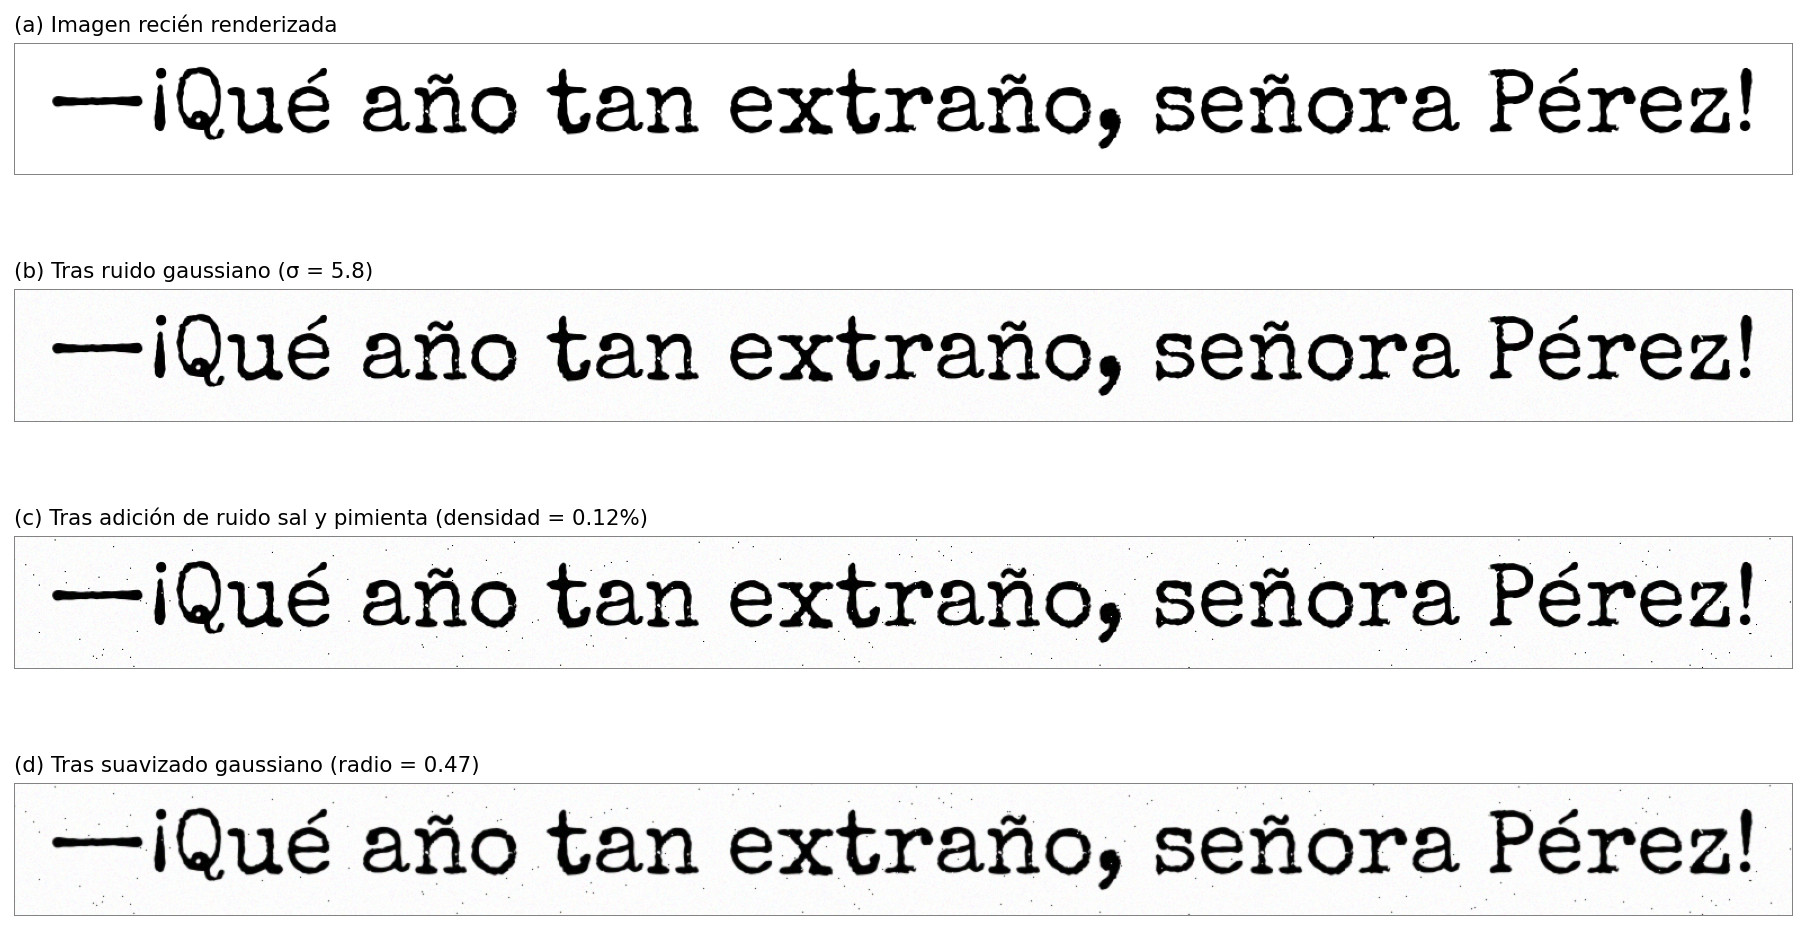
\includegraphics[width=\textwidth]{Graphics/degradacion_visual.png}
	\caption{Etapas acumulativas de la simulación de degradación visual sobre una línea recién renderizada del \textit{corpus} sintético, con la fuente SpecialElite. El panel~(a) muestra la imagen original tras el renderizado. El panel~(b) muestra la imagen tras la adición de ruido gaussiano con desviación típica~$\sigma$. El panel~(c) muestra la imagen tras la adición posterior de ruido sal y pimienta. El panel~(d) muestra la imagen tras el suavizado gaussiano final, que el sistema aplica al 50\,\% de las imágenes que escoge al azar. Los parámetros concretos que cada panel reporta corresponden a una realización aleatoria con los rangos que el texto describe.}
	\label{fig:degradacion-visual}
\end{figure}

La compatibilidad con ambos métodos de binarización es la propiedad que justifica la elección de las tres transformaciones y excluye otras alternativas. Otsu~\cite{otsu1979threshold} calcula un umbral global a partir del histograma bimodal de la imagen completa; Sauvola~\cite{sauvola2000binarization} calcula un umbral local para cada píxel a partir de la media y la desviación típica de los valores de gris en una vecindad. Las tres transformaciones modifican las estadísticas de niveles de gris de forma acotada y controlada, lo que permite a ambos métodos producir una binarización coherente sin perder caracteres. Transformaciones que alteren la geometría de los caracteres, como deformaciones elásticas o rotaciones agresivas, romperían la correspondencia entre la imagen y su transcripción y producirían etiquetas incorrectas. El capítulo~\ref{chap:preprocesamiento} ofrece la descripción de los dos métodos de binarización y del criterio de selección automática.

% -----------------------------------------------------------------------------
\section{Vocabulario indexado del sistema}
\label{sec:vocabulario}

El vocabulario de un sistema OCR es el conjunto cerrado de símbolos que el modelo puede producir como salida, cada uno asociado a un índice numérico. En cada paso temporal, la red CRNN produce un vector de probabilidades cuya dimensión coincide con el tamaño del vocabulario más uno. El paso adicional corresponde al \textit{token blank} propio de la función de pérdida CTC, que el capítulo~\ref{chap:modelo} describe.

El vocabulario del sistema comprende cien símbolos producibles, que el trabajo organiza de acuerdo con las convenciones de los marcos de entrenamiento OCR con CTC. La organización es la siguiente:

\begin{itemize}
	\item El índice cero corresponde al espacio en blanco, colocado en primera posición por ser el carácter más frecuente en cualquier texto corrido.
	\item Los índices uno a treinta y tres corresponden a las letras minúsculas del español, ordenadas por frecuencia objetivo descendente.
	\item Los índices treinta y cuatro a sesenta y seis corresponden a las letras mayúsculas en el mismo orden.
	\item Los índices sesenta y siete a setenta y seis corresponden a los dígitos del cero al nueve.
	\item Los índices setenta y siete a noventa y nueve corresponden a los signos de puntuación y a los símbolos tipográficos, ordenados también por frecuencia objetivo descendente.
	\item El índice cien queda reservado para el \textit{token blank} de CTC, que el marco de entrenamiento gestiona internamente sin que el modelo lo produzca como símbolo.
\end{itemize}

La organización por frecuencia objetivo descendente no es arbitraria. Algunos marcos de entrenamiento inicializan los sesgos de la capa de salida en función del índice, y mantener los símbolos más frecuentes con índices bajos puede acelerar la convergencia en las primeras épocas. La asignación explícita del índice cien al \textit{blank}, en lugar del índice cero como en algunos marcos, es una decisión consistente con el marco de entrenamiento que el sistema adopta. El capítulo~\ref{chap:modelo} ofrece la descripción del marco.

Al definir el vocabulario y generar el \textit{corpus}, el último paso del trabajo que el presente capítulo describe consiste en verificar las propiedades estadísticas del resultado.

% -----------------------------------------------------------------------------
\section{Análisis exploratorio del \textit{corpus} generado}
\label{sec:eda-corpus}

El análisis exploratorio del \textit{corpus} verifica que el resultado del procedimiento de generación satisface las propiedades de diseño que las secciones anteriores describen. El trabajo aplica el procedimiento a todo \textit{corpus} que el generador produce, antes de considerarlo apto para entrenamiento. La presente sección documenta el procedimiento y reporta los resultados sobre el \textit{corpus} de entrenamiento del sistema, que reúne 19\,998 imágenes que el generador produce con las nueve fuentes tipográficas que la subsección~\ref{subsec:fuentes-entrenamiento} describe. El procedimiento de análisis es idéntico para cualquier \textit{corpus} que el generador produzca, con independencia del repertorio tipográfico que emplee.

El análisis cubre cinco dimensiones: distribución de imágenes entre fuentes, longitudes de etiqueta, dimensiones de imagen, cobertura del vocabulario y frecuencias de caracteres. La figura~\ref{fig:eda-dashboard} reúne las visualizaciones del análisis en un único panel.

\begin{figure}[!htbp]
	\centering
	
\includegraphics[width=0.85\textwidth]{Graphics/eda_dashboard.png}
	\caption{Análisis exploratorio del \textit{corpus} sintético de entrenamiento, con 19\,998 imágenes que el generador produce a partir de las nueve fuentes tipográficas seleccionadas. El panel reúne las distribuciones de imágenes por fuente, longitudes de etiqueta, anchos, frecuencias de caracteres, cobertura del vocabulario español, cumplimiento de la restricción CTC, alturas por fuente y aspect ratio de las imágenes.}
	\label{fig:eda-dashboard}
\end{figure}

La distribución de imágenes entre fuentes resultó perfectamente uniforme, con 2\,222 imágenes por cada una de las nueve fuentes y un cociente entre la frecuencia máxima y la mínima igual a la unidad. La uniformidad garantiza que ninguna fuente tipográfica recibe más peso que las demás durante el entrenamiento.

Las longitudes de etiqueta presentaron una media de 38,5 caracteres, mediana de 37 caracteres y rango entre 9 y 74 caracteres, con desviación típica de 13,8 caracteres. Los percentiles 5, 25, 75 y 95 fueron 19, 28, 48 y 64 caracteres, respectivamente. La distribución resultó suave, sin acumulaciones en los extremos, gracias al sorteo aleatorio de la longitud máxima por cadena que la subsección~\ref{subsec:cadenas-balanceadas} describió.

Las dimensiones de imagen presentaron media de ancho de 1\,704 píxeles, mediana de 1\,630 píxeles, rango entre 229 y 3\,616 píxeles, y coeficiente de variación del 37,9\,\%. La altura la determinan el tamaño de fuente fijo y los márgenes, y presentó una media de 121 píxeles y rango entre 79 y 142 píxeles. La variabilidad del ancho es coherente con el rango de longitudes de etiqueta y con la diferencia de ancho entre fuentes monoespacio y fuentes serif para textos de la misma longitud. El análisis verificó el cumplimiento de la restricción que la función de pérdida CTC impone por inspección directa de cada par imagen--etiqueta: ninguna de las 19\,998 imágenes viola la restricción, según la cual el ancho de la imagen debe ser mayor o igual que la longitud de la etiqueta multiplicada por el factor de reducción horizontal de la red convolucional. El capítulo~\ref{chap:modelo} describe el detalle de la restricción.

La cobertura del vocabulario fue total: los cien símbolos del vocabulario del sistema están presentes en el \textit{corpus}, y ningún carácter del \textit{corpus} queda fuera del vocabulario. El \textit{corpus} reúne 770\,027 caracteres distribuidos en 147\,825 palabras, de las cuales 15\,001 son únicas. El coeficiente de variación de las frecuencias de caracteres alcanzó el 203,2\,\%, valor esperable en lenguaje natural dada la ley de Zipf~\cite{zipf1949human} que el capítulo~\ref{chap:estado-arte} introdujo.

Los caracteres específicos del español formal cubren todos el umbral mínimo de 500 apariciones. Las vocales con tilde (á, é, í, ó, ú) y la diéresis presentaron entre 1\,986 y 4\,705 apariciones cada una. La eñe alcanzó 3\,343 apariciones, las comillas angulares 3\,338 y 3\,335, y la raya de diálogo 6\,052. Los signos de apertura de interrogación y exclamación superaron 3\,300 apariciones cada uno. Tres símbolos genéricos quedaron por debajo del umbral: el corchete izquierdo (85 apariciones), el corchete derecho (83) y la almohadilla (87). Los tres son símbolos de uso poco frecuente en el español formal y no figuran entre los caracteres específicos del idioma. El procedimiento de generación los incluye en el vocabulario por exhaustividad, sin priorizar su sobremuestreo por encima de los caracteres del español. La métrica de cobertura mínima por carácter, que cubre los símbolos propios del idioma, resulta satisfactoria.

El análisis exploratorio confirma que el procedimiento de generación produce un \textit{corpus} conforme al diseño: balanceado entre fuentes, con longitudes de etiqueta en un rango operativo, con la representación total del vocabulario, con todos los caracteres específicos del español cubiertos por encima del umbral mínimo, y sin pares imagen--etiqueta que violen la restricción de la función de pérdida CTC.

% -----------------------------------------------------------------------------
% Transición al capítulo 3
% -----------------------------------------------------------------------------

Con el \textit{corpus} ya generado, validado y conforme al diseño, el capítulo cierra. El capítulo siguiente aborda la segunda contribución técnica del trabajo: el \textit{pipeline} de preprocesamiento que transforma documentos digitalizados reales en una secuencia de líneas de texto que sigue el formato que el modelo de reconocimiento espera.
